\documentclass[a4paper,10pt]{article}
\usepackage[top=15mm,bottom=15mm,left=16mm,right=16mm]{geometry}
\usepackage{luatexja-fontspec}
\setmainfont{DejaVu Serif}
\setsansfont{DejaVu Sans}
\setmainjfont{Noto Serif CJK JP}
\setsansjfont{Noto Sans CJK JP}
\usepackage{fix-cm}
\usepackage{graphicx,xcolor,booktabs,amsmath,amssymb,array,caption,fancyhdr}
\usepackage[colorlinks=true,linkcolor=teal,urlcolor=teal,citecolor=teal]{hyperref}
\definecolor{teal}{HTML}{126D70}
\definecolor{ink}{HTML}{182F40}
\definecolor{muted}{HTML}{516574}
\hypersetup{pdftitle={3DGSによる視点拡張と幾何教師を用いたテニスコート検出},pdfauthor={tennis-lab},pdfsubject={Method and qualitative evaluation with four supplied photographs}}
\setlength{\parindent}{1em}
\setlength{\parskip}{1.3mm}
\setlength{\tabcolsep}{3mm}
\renewcommand{\arraystretch}{1.15}
\captionsetup{hypcap=false,font=small,labelfont=bf,labelsep=quad,skip=2mm}
\renewcommand{\figurename}{図}
\renewcommand{\tablename}{表}
\renewcommand{\refname}{参考文献}
\pagestyle{fancy}\fancyhf{}\renewcommand{\headrulewidth}{0pt}
\fancyfoot[L]{\sffamily\fontsize{7}{9}\selectfont\color{muted}TENNIS-LAB / Court detection / 2026-09-19}
\fancyfoot[R]{\sffamily\fontsize{8}{10}\selectfont\thepage}
\newcommand{\sect}[1]{\section{#1}\vspace{-1mm}}
\newcommand{\panel}[2]{\begin{minipage}[t]{.326\linewidth}\centering\sffamily\fontsize{7.2}{9}\selectfont #2\par\vspace{.6mm}\includegraphics[width=\linewidth]{figures/#1}\end{minipage}}
\newcommand{\epanel}[2]{\begin{minipage}[t]{.326\linewidth}\centering\sffamily\fontsize{7.2}{9}\selectfont #2\par\vspace{.6mm}\includegraphics[width=\linewidth,height=32mm,keepaspectratio]{figures/#1}\end{minipage}}
\newcommand{\external}[1]{%
\noindent\epanel{#1_input.png}{入力写真}\hfill\epanel{#1_baseline.png}{TCD：局所補正KP（Hなし）}\hfill\epanel{#1_ours.png}{本モデル：KP14＋H}\par\vspace{1mm}
\noindent\epanel{#1_ours_line_mask.png}{本モデル：LINE二値マスク}\hfill\epanel{#1_ours_line_overlay.png}{本モデル：LINE重畳 $p\geq0.5$}\hfill\epanel{#1_ours_heat.png}{本モデル：LINE確率 $[0,1]$}\par}
\newcommand{\scenerow}[7]{\noindent{\sffamily\bfseries #1}\par\vspace{.5mm}\panel{#2}{#3}\hfill\panel{#4}{#5}\hfill\panel{#6}{#7}\par\vspace{.8mm}}

\begin{document}
\begin{center}
{\sffamily\bfseries\fontsize{17}{23}\selectfont\color{ink}3DGSによる視点拡張と幾何教師を用いた\\テニスコート検出}\par\vspace{2mm}
{\fontsize{10}{14}\selectfont データ生成・多タスク学習・未学習画像での定性評価}\par\vspace{2mm}
{\sffamily\fontsize{8}{11}\selectfont tennis-lab\quad 技術報告\quad 2026年9月19日}
\end{center}\par
\vspace{-1mm}
\begin{abstract}
放送映像に偏ったコート検出器を、多様な撮影視点へ適用するための実装済みパイプラインを整理する。
実動画から3D Gaussian Splatting（3DGS）でシーンを再構成し、地面と規格コートを位置合わせして、新規視点のRGBと幾何教師を生成する。
これを実画像と混合し、凍結DINOv3特徴にTransformer・DPT・複数の予測ヘッドを接続して学習する。
指定された写真4枚で既存重みを推論した結果、LINE出力はコートの線構造を捉える一方、キーポイントからのホモグラフィ復元にはずれが残った。
B00--B03各3視点の実レンダリングと全4枚の推論を掲載する。
本報告の「未学習」は指定写真を下流学習へ追加していないことを指し、事前学習との非重複を保証しない。
人手正解を持たない定性比較のため、精度向上や合成データ単独の効果は主張しない。
\end{abstract}

\sect{はじめに}
テニスシーンの3次元再構成では、コートの規格寸法がボール・プレーヤーの位置を共通座標系に結び付ける基準になる。
しかし、固定された放送視点での検出が良好でも、低い視点、横向き、見切れ、背景の変化に対応できるとは限らない。
必要なのは、\emph{線が見えること}と\emph{正しい規格コートへ対応付くこと}を分けて確かめることである。
本報告は、既存の再構成・教師生成・学習を一つの手法として記述し、生成画像上の幾何整合と指定実画像上の推論を追跡可能な形で示す。
新規の学習や再構成は実施せず、保存成果物と重みを用いる。

\sect{関連研究}
TennisCourtDetector（TCD）\cite{tcd}はTrackNetに近い構成で14点のコートキーポイント（KP）を推定し、局所的な線検出とホモグラフィで補正する。
3DGS\cite{gs}は異方性Gaussianの位置・形状・不透明度・外観を最適化し、校正カメラに対する新規視点画像を合成する。
本手法ではこの画像合成を教師付きデータの視点拡張に用いる。
検出器には自己教師あり視覚特徴のDINOv3\cite{dino}と、多段特徴を空間的な予測へ戻すDPT\cite{dpt}を組み合わせる。
これら自体の新規性ではなく、規格コートの幾何と実画像の教師を接続する構成が本報告の対象である。

\sect{手法}
\subsection{3DGS再構成と規格コートへのアライメント}
動画の多視点画像からSfMでカメラの内部・外部パラメータとシーンを推定し、3DGSの学習済み表現を得る。
再構成座標のスケールは任意なので、規格コートの長さ23.77 m・ダブルス幅10.97 mを尺度とする。
再構成点のRANSAC平面推定（図\ref{fig:ransac}）とLINE検出の地面への投影（図\ref{fig:projection}）を使い、共通スケールと各コートの平面内位置・向きを求める。
推定地面 $\mathbf n^\top(\mathbf X-\mathbf o)=0$ に対し、カメラ中心 $\mathbf C$、画素からのレイ $\mathbf d$ の交点は
\begin{equation}
\mathbf X=\mathbf C+\lambda\mathbf d,\qquad
\lambda=\frac{\mathbf n^\top(\mathbf o-\mathbf C)}{\mathbf n^\top\mathbf d}
\end{equation}
となる。平面に平行・カメラ後方などの無効な交差は除外する。
各視点のLINE確率を共通の地面グリッドへ写像し、距離に応じた重みで集約する。
その証拠に規格コートを当てはめ、残差から追加コートを探索する。
当てはめ用と保留視点を分け、検出線との距離・支持量で整合性を確認する。
保存結果のB00・B03は自動受理、B01・B02は人手調整・確認を含む。
したがって、全シーンが自動処理だけで得られたものではない。

\newpage
\noindent\textbf{地面推定と多視点LINE投影の実例（B00）}\par
{\small
カメラの上方向・撮影範囲・高さ分布から点群の地面候補を絞り、3点から作る平面を1,000回試す。
最大20,000候補点の距離内支持数を最大化し、同数なら残差中央値の小さい仮説を選ぶ。
その後、支持点のSVDによる平面再推定を3回行う。
元の217,407点と保存設定（seed 42）から再計算し、保存平面との一致を確認した。
}\par
\noindent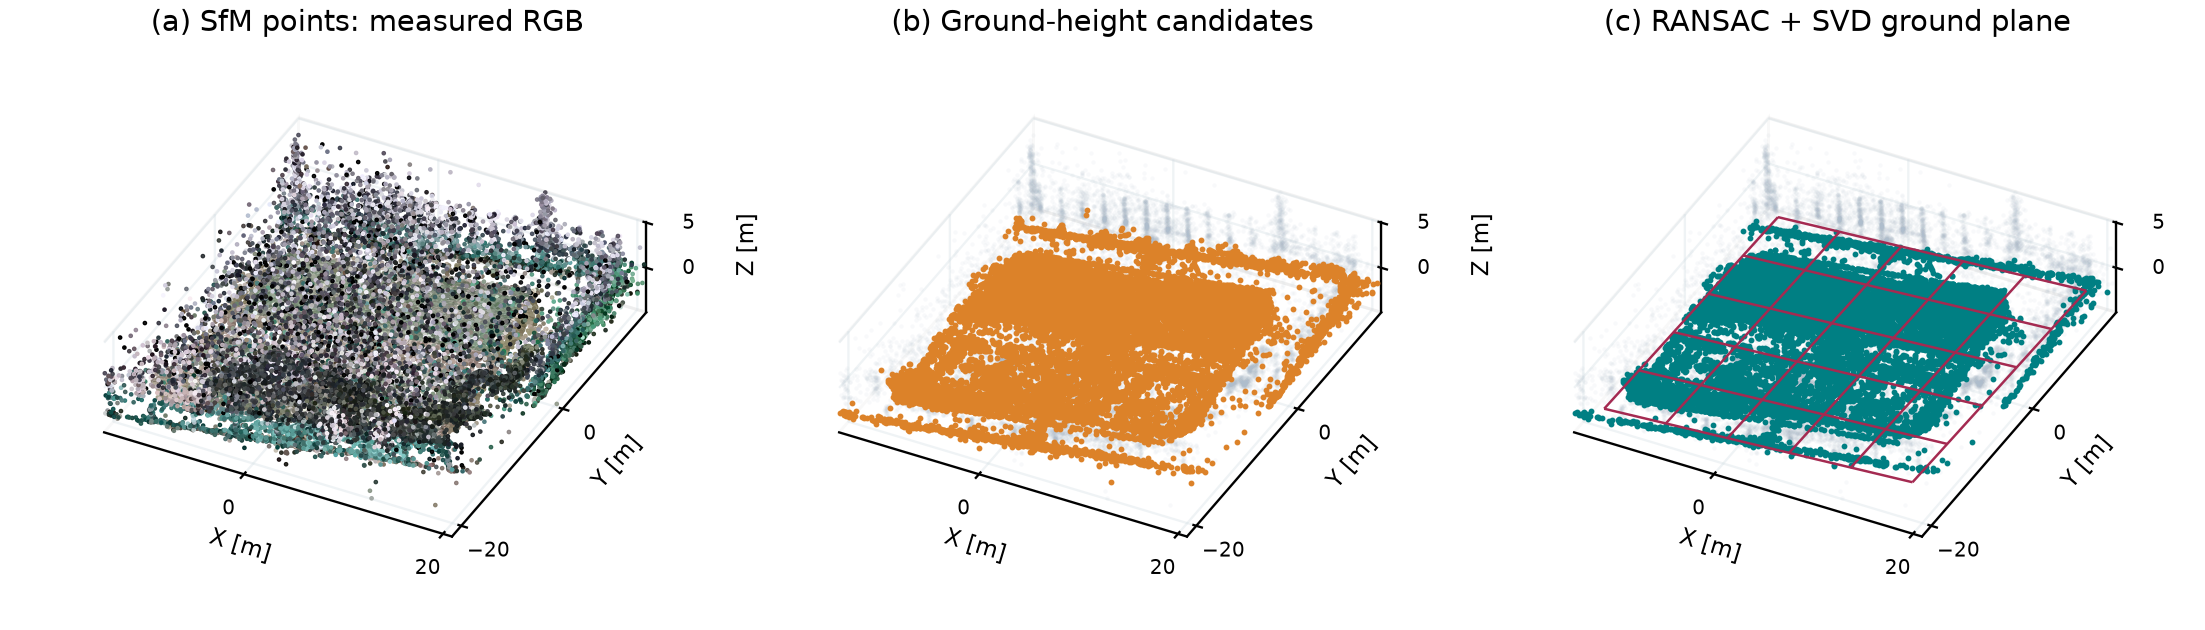
\includegraphics[width=\linewidth]{figures/method_ransac.png}
\captionof{figure}{実SfM点群からの地面推定。(a)元のRGBを持つ点群、(b)高さ帯の候補75,208点（橙）、(c)RANSAC＋SVD後の支持65,325点（青緑）と推定平面（赤紫）。距離しきい値は再構成座標でRANSAC 0.006、再推定0.008。軸は確定スケールでmへ換算した。3パネルは同じ地面周辺領域を拡大し、表示のみ3点に1点へ間引き、候補・支持点を前面に描いた。表示の切り出し・間引きは推定に影響しない。}\label{fig:ransac}\par
\vspace{1mm}
{\small
LINE確率$p\geq0.5$の画素をレイと地面の交点へ写し、共通グリッド（約3.58 cm）に配置する。
距離$r$による重み$w=1/(1+(r/5.01\,\mathrm m)^2)$を用い、各視点・各セルで$e_v(g)=\max_{x\mapsto g}w_v(x)p_v(x)$、
全当てはめ視点の証拠を$E(g)=\sum_{v\in\mathrm{fit}}e_v(g)$とする。$E$は確率ではなく重み付きの総量である。
}\par
\noindent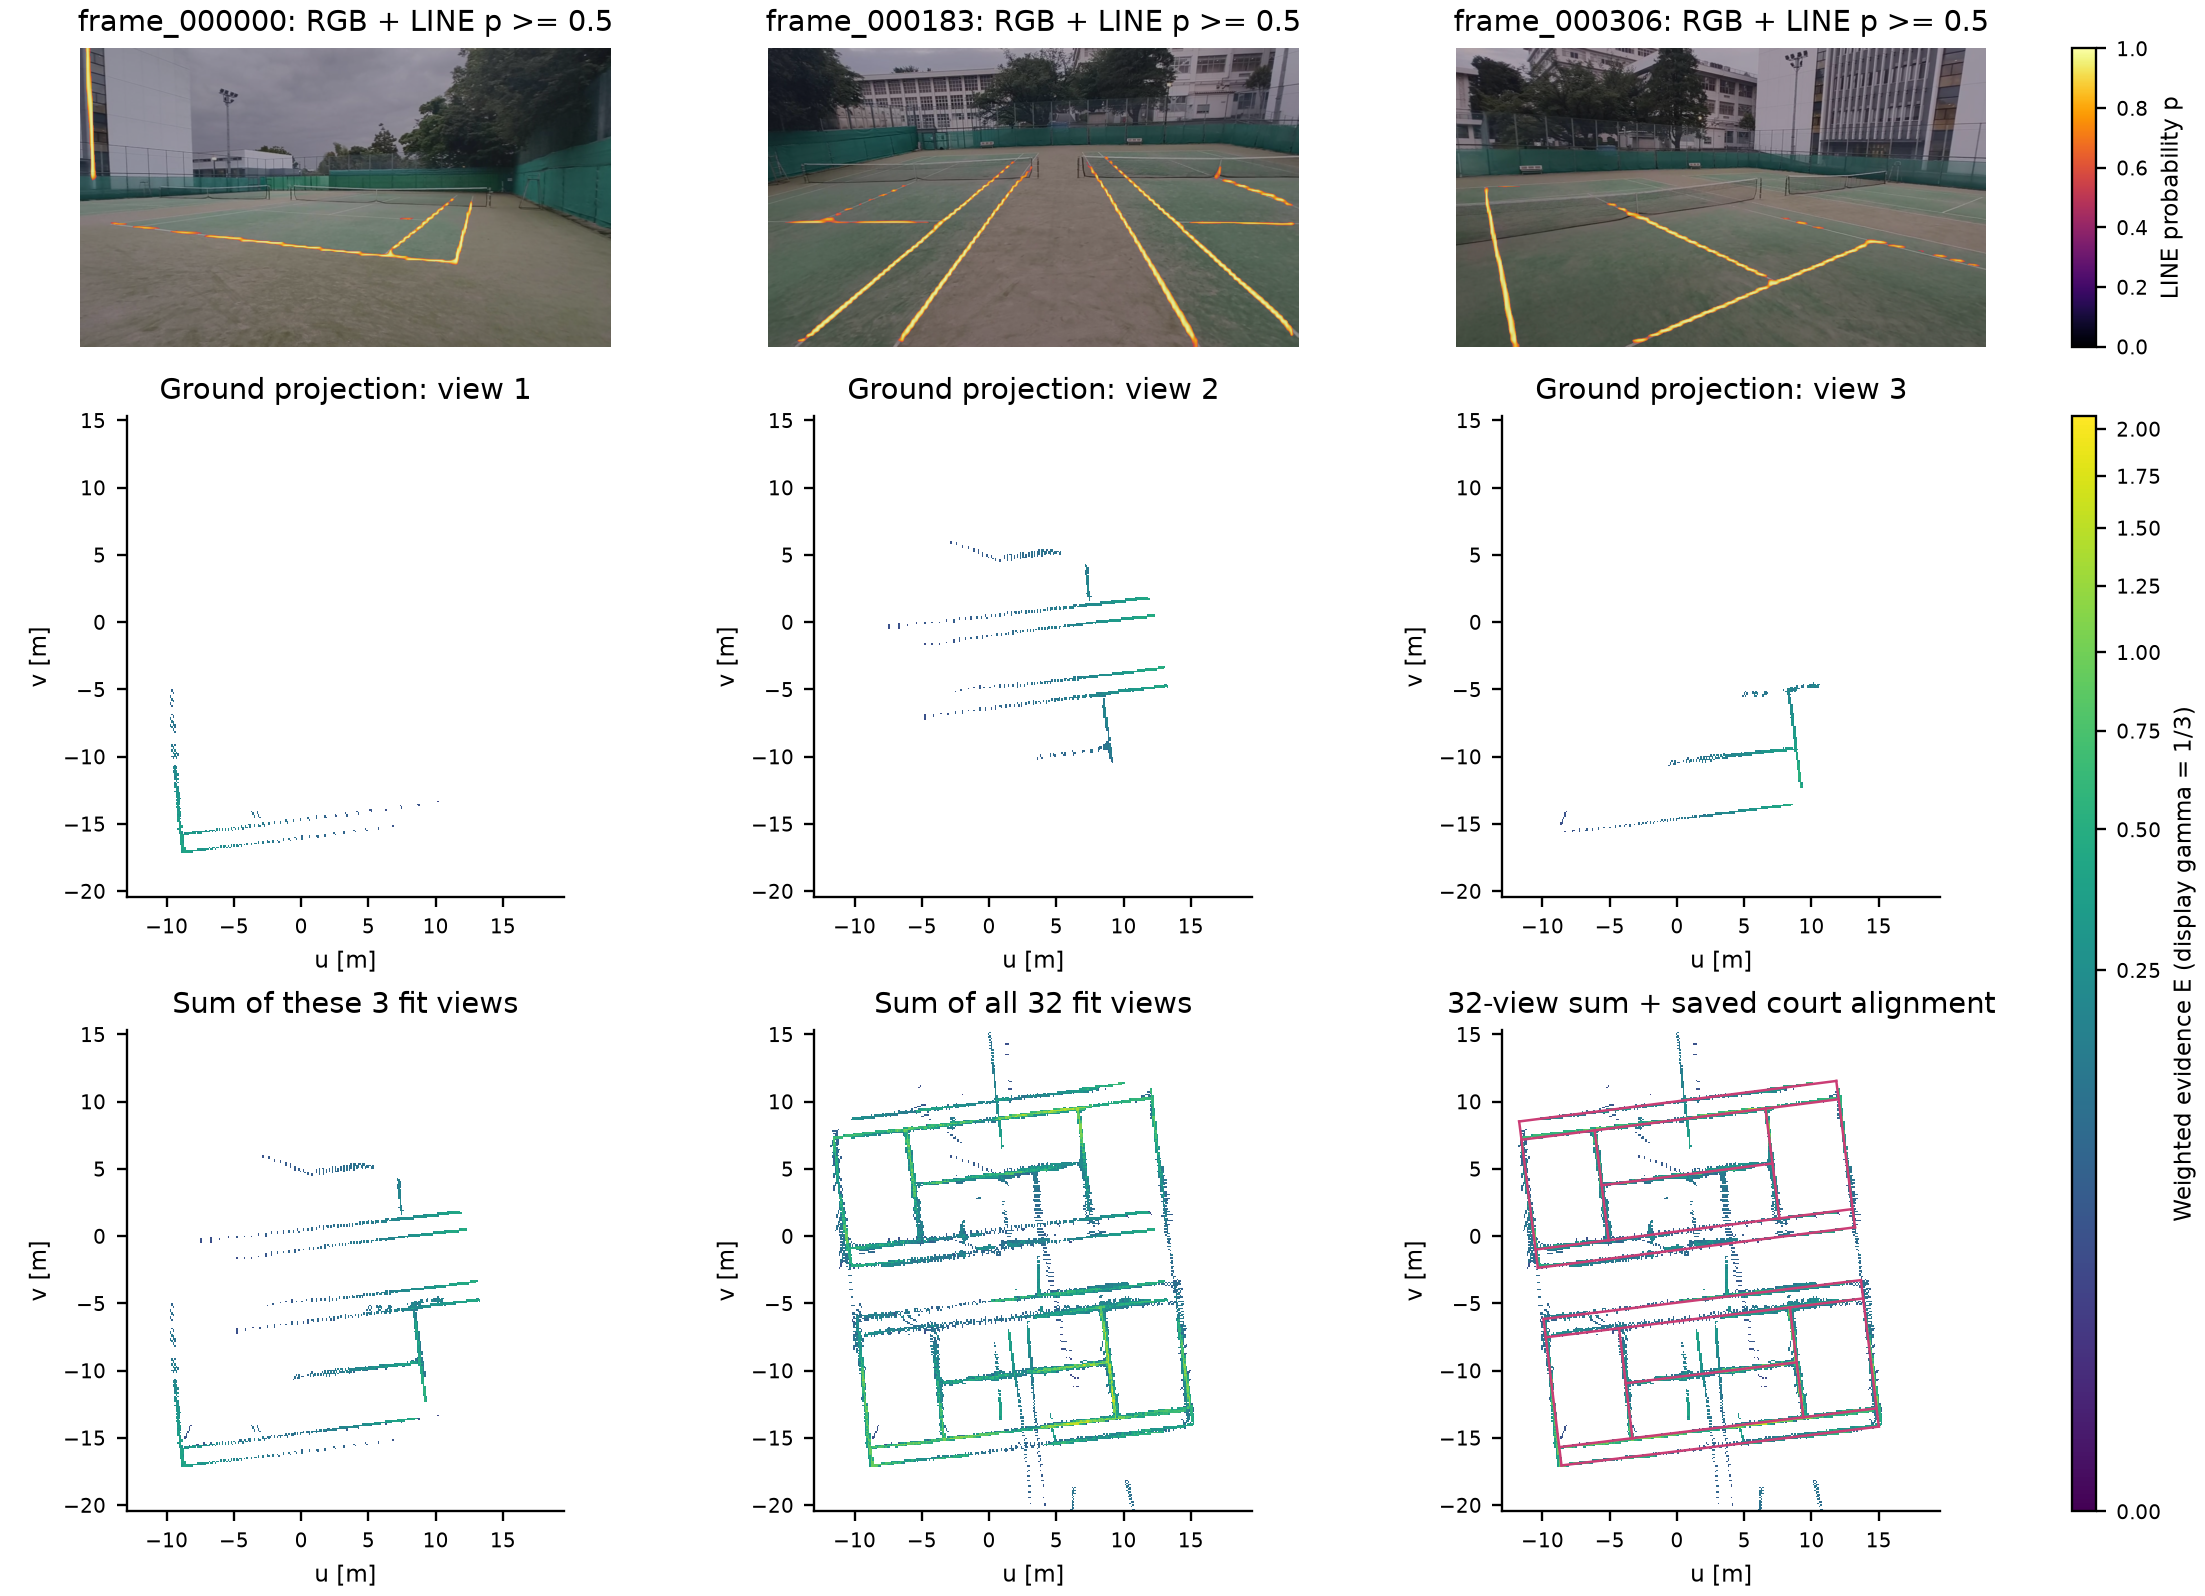
\includegraphics[width=\linewidth]{figures/method_projection.png}
\captionof{figure}{各視点のLINEから投影・集約への過程。上段は校正済み実画像と実LINE確率の重畳、中段は同じ地面座標への各視点の投影。下段は表示3視点の和、全32当てはめ視点の和、保存コートとの重畳。16保留視点は集約に含めない。地面図は白が支持なし、色域共通。細線を読めるよう表示のみ$3\times3$セルの最大値へ縮約し、$\gamma=1/3$とした。元の集約グリッドは保存値と完全一致した。当時の実画像入力・LINE専用重み（epoch 19）の結果であり、未学習推論用の多タスク重み（epoch 17）とは区別する。}\label{fig:projection}

\newpage
\subsection{新規視点画像と教師の生成}
コート中心を向く複数のカメラ軌道を設定し、3DGSからRGBをレンダリングする。
規格コート点 $\mathbf X_j^c$ をシーンへ移す変換を $T_{s\leftarrow c}$、カメラ姿勢を $T_{s\leftarrow v}$ とすると、同じ視点の教師画素は
\begin{equation}
\widetilde{\mathbf u}_{vj}\sim
K_v\,[I\mid0]\,T_{s\leftarrow v}^{-1}T_{s\leftarrow c}
\begin{bmatrix}\mathbf X_j^c\\1\end{bmatrix}
\end{equation}
で求める。レンダリングと教師でカメラ・座標系を共有することが整合の要点である。
保存データのv3契約は対象コート1面・KP14で、反対側の視点では近遠・左右の対応を180度回転の規則で揃える。
画面内・前方・レンダラでの可視性を区別し、KPヒートマップ、領域分割（SEG）、二値LINE、線種ごとのsemantic LINEを構成する。
連続した近接画像の混入を避けるため分割は軌道群単位とする。ただし同じ会場が各分割に含まれるため、会場分離の評価ではない。

\subsection{検出器と学習目的}
凍結したDINOv3 ViT-B/16の第3・6・9・12ブロック特徴を利用する。
最深段に幅768・8層・12ヘッドのTransformerを挿入し、その空間特徴と浅い3段を512チャネルのDPTで融合する。
各密予測ヘッドは256チャネル・3残差ブロックからなり、KP、SEG、LINE、semantic LINEを出力する。
別のqueryから姿勢を推定する10次元ヘッド（回転6次元、並進3次元、対数焦点距離1次元）も学習する。
損失は
\begin{equation}
\mathcal L=\mathcal L_{\rm KP}
+\mathcal L_{\rm SEG}+\mathcal L_{\rm LINE}
+\mathcal L_{\rm SLINE}+\mathcal L_{\rm pose}^{\rm synth}
\end{equation}
であり、KPはfocal BCE（$\gamma=2$）、領域・線種はCE＋Dice、LINEは正例重み8のBCE＋Diceを用いる。
姿勢は合成画像だけに教師を持ち、並進MSE・回転の測地角・対数焦点距離MSEを等重みで加える。
KPと姿勢の整合損失はこの重みでは無効である。
各バッチを合成4枚＋TCD実画像4枚とし、短辺256/320/384/448/512の多解像度、色変動・ぼかしで学習した。
AdamW、学習率$10^{-4}$、weight decay 1、warmup 3 epochを用いた保存重み（epoch 17、29,844 step）を固定する。
本報告の写真に対する再学習・重み選択は行わない。

\sect{実験設定と評価範囲}
\subsection{データと「未学習」の確認}
指定フォルダ内の4ファイルを名前順でA--Dに対応付け、すべて推論・掲載した（図\ref{fig:ab}、\ref{fig:cd}）。
TCDの8,841枚とB00--B03の8,415レンダリングを照合し、ファイルSHA-256および向き補正後RGBの完全一致は0件だった。
知覚ハッシュによる類似性検査も保存したが、これらは別撮影や同会場、非公開の事前学習集合との重複まで否定するものではない。
撮影者・撮影日・原公開URLは入力に付属しておらず、会場名は推測していない。

\subsection{比較条件と表示方法}
TCDは公開重みとBGR入力640$\times$360、しきい値170/255の公式ピーク抽出・局所補正を用いる。
本モデルはRGB・ImageNet正規化、短辺512・16画素整列で推論し、KPをチャネルごとに1点抽出する。
両者のKPにTCDの12種類の4点組によるホモグラフィ候補選択を適用する。
候補は残りの観測点への平均誤差で選び、特異行列や評価点のない候補は採用しない。
TCDの補正・H推定は1280$\times$720座標で行い、原画像へ戻す。
加えてTCDの14チャネルargmaxでのH生成可否を数表に併記し、しきい値による棄却の影響を確認する。

指定写真4枚とTCD動作確認の推論はCPU、EXIF補正は共通、追加クロップなしとした。
本モデルのLINEは確率0.5以上を白とする二値マスク・原画像への直接重畳・確率マップの3形式で示す。確率マップは共通の$[0,1]$色域を使う。
\textbf{Hの生成可否や検出点数は正解率ではない。}画像に人手GTはなく、LINEを持たないTCDとの出力差、backbone・解像度・学習データの差も残る。
TCDの既存val画像1枚では14点を検出し、H補正後の平均誤差1.423 pxを確認した。これは実装の動作確認であり、外部4枚の評価には含めない。

\newpage
\sect{結果}
\subsection{3DGSレンダリングと保存アライメント}
\begin{minipage}{\linewidth}
\scenerow{B00：2面 / 自動受理}{B00_000720_alignment.png}{sample 000720}{B00_001493_alignment.png}{sample 001493}{B00_000423_alignment.png}{sample 000423}
\scenerow{B01：3面 / 人手確認}{B01_001403_alignment.png}{sample 001403}{B01_001918_alignment.png}{sample 001918}{B01_001601_alignment.png}{sample 001601}
\scenerow{B02：1面 / 人手確認}{B02_000808_alignment.png}{sample 000808}{B02_001982_alignment.png}{sample 001982}{B02_000445_alignment.png}{sample 000445}
\scenerow{B03：1面 / 自動受理}{B03_001112_alignment.png}{sample 001112}{B03_001091_alignment.png}{sample 001091}{B03_001288_alignment.png}{sample 001288}
\captionof{figure}{実際の3DGS新規視点レンダリングに、保存済み3Dコートを同じカメラで再投影した12例。各行は異なる3軌道群から、線構造と視点差を確認できる例を選んだ。色はシーン内のコート識別（水色・橙・桃）であり、予測の確信度ではない。全コートの地面線を描き、ネット等による遮蔽マスクは適用していない。ぼけ・浮遊物・見切れも元レンダリングのまま残した。}\label{fig:gs}
\end{minipage}\par
\vspace{2mm}
\begin{center}\small
\begin{tabular}{@{}lrrrrl@{}}\toprule
 & train & val & test & 軌道群 & 保留視点の整合RMS [m]\\\midrule
B00 & 1,718 & 220 & 238 & 35 & 0.105 / 0.130\\
B01 & 1,559 & 295 & 198 & 26 & 0.032 / 0.233 / 0.036$^*$\\
B02 & 1,648 & 194 & 252 & 40 & 0.091$^*$\\
B03 & 1,669 & 226 & 198 & 40 & 0.109\\\midrule
計 & 6,594 & 935 & 886 & 141 & \\\bottomrule
\end{tabular}
\captionof{table}{保存済み生成データの内訳とコートごとの整合値。RMSは測量正解への誤差ではなく、検出された線との残差。$^*$人手調整後の参考値であり、独立な自動検証値として比較しない。}\label{tab:data}
\end{center}\par
\vspace{-2mm}
{\small 図\ref{fig:gs}の3D座標・カメラによる再投影は、保存された2D教師と照合した。これは成果物同士の一貫性の検証であり、教師そのものが物理的に正しいことの保証ではない。B00・B03の自動当てはめは各32視点、保留は各16視点である。}

\newpage
\subsection{指定実画像への推論：低視点・斜視}
{\small 橙＝TCD、水色＝本モデル。KP＋H欄の点は抽出KP、線はそのKPから求めた規格コート投影。TCD公式欄の点は局所補正後。Hなしの場合は点だけを表示する。LINE欄はテンプレートを当てはめていない直接の密予測である。}\par
\vspace{1mm}
\noindent\textbf{A：\texttt{ennai011\_1.jpg} / 1,000$\times$667}\par
\external{local01}
{\small TCDの公式処理は3点でHを生成できず、argmaxに変えても大きく崩れた配置となる。本モデルのLINEは外周・内側線を捉える。KP＋Hは輪郭の一部に沿うものの、奥側の点の対応や内側線にはずれが見られる。}\par
\vspace{3mm}
\noindent\textbf{B：\texttt{images (1).jpg} / 638$\times$480}\par
\external{local02}
{\small TCDは公式処理で1点、argmaxでも有効なHを生成できない。本モデルは画面右へ見切れる線を含めてLINEを検出するが、KP＋Hは手前側の輪郭と一致しない。線の抽出と点の意味的対応付けの差が現れている。}
\captionof{figure}{指定写真A・Bの実推論。上段でKPと幾何復元、下段で本モデルのLINE出力を示す。二値マスクは白が$p\geq0.5$、黒がそれ未満。確率マップは黒0から黄白1までの固定色域。全パネルは縦横比を保ち、元画像の全領域を表示した。}\label{fig:ab}\par
\vspace{2mm}
\begin{center}\small
\begin{tabular}{@{}lrrrr@{}}\toprule
 & A & B & C & D\\\midrule
TCD公式：検出点数 / 14 & 3 & 1 & 0 & 1\\
TCD公式：H生成 & 不可 & 不可 & 不可 & 不可\\
TCD argmax：H生成 & 可 & 不可 & 不可 & 不可\\
本モデル：KP数 / H生成 & 14 / 可 & 14 / 可 & 14 / 可 & 14 / 可\\\bottomrule
\end{tabular}
\captionof{table}{保存推論から集計した出力の状態。しきい値とデコード方式が違うため、点数を両モデルの精度比較に用いることはできない。Hが生成されても正しい対応とは限らない。}
\end{center}

\newpage
\subsection{指定実画像への推論：人物・観客席を含む場面}
\noindent\textbf{C：\texttt{images (2).jpg} / 547$\times$365}\par
\external{local03}
{\small 本モデルのLINEはコートに沿って反応するが、手前や人物周辺に途切れがある。KP＋Hではコートの奥行きが縮み、手前の領域を復元できていない。TCDは公式処理で0点、argmaxでもHを生成できない。}\par
\vspace{2mm}
\noindent\textbf{D：\texttt{images.jpg} / 678$\times$452}\par
\external{local04}
{\small 本モデルは俯瞰の線構造を捉える一方、画面下にも小さなLINE反応がある。KP＋Hは特に奥側・左側の線で実コートとずれる。TCDは公式処理で1点、argmaxでもHを生成できない。}
\captionof{figure}{指定写真C・Dの実推論。表示条件は図\ref{fig:ab}と共通。4例とも、本モデルのLINEとKP由来の幾何復元は同じ品質にはなっていない。}\label{fig:cd}\par
\section{課題点}
\subsection{SfMのドリフトと幾何教師への影響}
SfMには、長い撮影区間で位置・姿勢・スケールの誤差が累積するドリフトの問題がある\cite{drift}。
再構成の変形は3DGSの外観と幾何教師の整合を損なうため、保存教師との再投影一致だけでは十分でない。
そこでB00の実SfM点217,407点と観測トラックを読み、491フレームを時系列で4等分して、地面の再構成高さを比較した（図\ref{fig:drift}）。

対象は保存コート2面の内側、推定地面から$\pm30$ cm以内、SfM再投影誤差1 px以下の点とした。
全観測が一つの区間に収まるトラックだけを使い、区間をまたぐ点は除く。
地面を0.5 m格子に分け、\textbf{全4区間で各5点以上を持つ共通33セル}に限定した。
各セル・各区間の高さ中央値から第1区間の値を引き、同じ領域同士の差を集計する。
これは同一特徴点の再推定比較ではなく、同一セル内の異なる点群による診断である。

\newpage
\noindent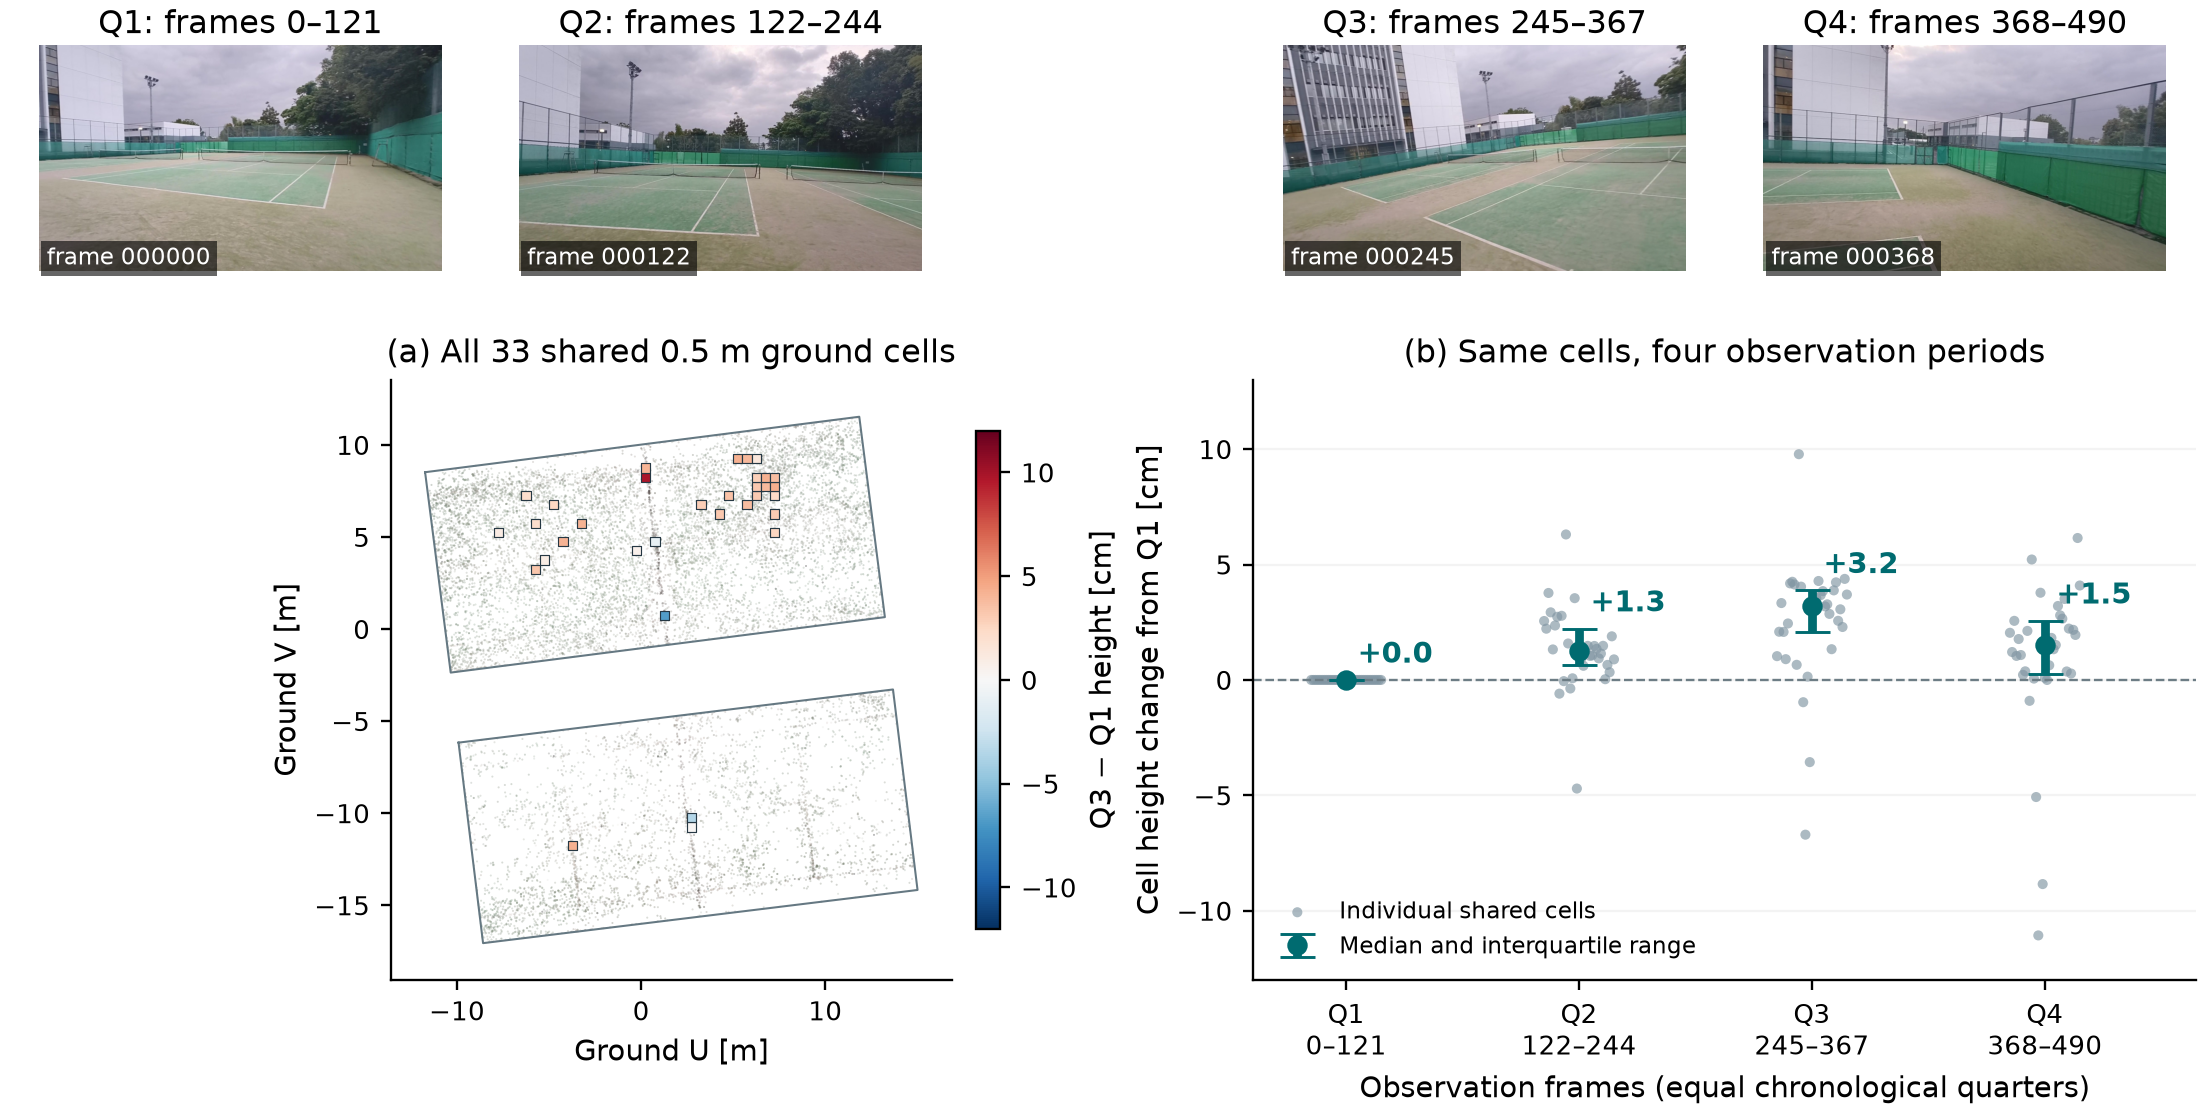
\includegraphics[width=\linewidth]{figures/sfm_temporal_drift.png}
\captionof{figure}{B00の実データによるドリフトの兆候。上段は各撮影区間の先頭の実画像。(a)元RGBを持つ地面点群と保存コート、共通33セルの位置・第3区間と第1区間の高さ差。(b)同じ33セルの区間別の差。灰点は全セル、青緑は中央値と四分位範囲であり、信頼区間ではない。点群の表示のみ3点に1点へ間引いた。m・cmへの換算には保存アライメントのスケールを使う。}\label{fig:drift}

第1区間に対する高さ差の中央値は、第2--4区間でそれぞれ\textbf{+1.3、+3.2、+1.5 cm}だった。
第3区間の四分位範囲は+2.1--+3.9 cmで、地面の高さが撮影区間に応じて偏る。
格子を1 mへ広げた感度確認でも、共通101セルにおける第3区間の中央値は+3.0 cmだった。
この時間依存の不整合はドリフトと整合する兆候だが、測量正解はなく、セル内の実際の凹凸や特徴点・三角測量の誤差とも分離できない。
したがって、\emph{絶対的なドリフト量の測定や、B00以外への一般化は行わない}。

一つの相似変換でコートをアライメントしても、区間ごとに異なる変形は取り除けない。
今後はSfM段階で地面の平面性や長距離の構造対応\cite{drift}を制約し、再訪時の対応と独立な地面基準で確認する必要がある。
これは、レンダリング枚数を増やす前に幾何教師の品質を確保する課題である。

\subsection{4シーンに限られる多様性と汎化性能の不足}
合成側はB00--B03の\textbf{4シーンのみ}で、8,415枚への視点拡張も、新しい会場・路面・照明・背景を追加するものではない。
TCD実画像8,841枚も混合しているが、合成側の分割は同一シーン内の軌道群単位であり、未知シーンへの汎化を測れていない。
また、4シーンを4つの独立した会場とみなすこともできない。

指定写真ではLINEが反応してもKP由来の規格コートはずれており、未知画像に対する幾何復元の汎化性能は十分でない。
ただし4枚・人手GTなしの観測から性能全体を定量化したり、シーン数だけを失敗原因と断定したりはできない。
会場・路面・照明の異なるシーンを追加し、会場を完全に分離した人手GT付き集合でLINEとKPを別々に評価する必要がある。
同一モデル・解像度で実写のみと合成混合を比較し、シーン数の増加が汎化へ与える効果も検証する。
\par
\vspace{-2mm}
\begin{thebibliography}{5}\fontsize{8}{10}\selectfont\setlength{\itemsep}{0mm}
\bibitem{tcd} yastrebksv. \href{https://github.com/yastrebksv/TennisCourtDetector}{TennisCourtDetector}. 公開コード・重み、コード版 e5cd4f1（2026-09-18参照）.
\bibitem{gs} B. Kerbl, G. Kopanas, T. Leimkühler, G. Drettakis. \href{https://repo-sam.inria.fr/fungraph/3d-gaussian-splatting/}{3D Gaussian Splatting for Real-Time Radiance Field Rendering}. ACM TOG 42(4), 2023.
\bibitem{dino} O. Siméoni et al. \href{https://arxiv.org/abs/2508.10104}{DINOv3}. arXiv:2508.10104, 2025.
\bibitem{dpt} R. Ranftl, A. Bochkovskiy, V. Koltun. \href{https://openaccess.thecvf.com/content/ICCV2021/html/Ranftl_Vision_Transformers_for_Dense_Prediction_ICCV_2021_paper.html}{Vision Transformers for Dense Prediction}. ICCV, 2021.
\bibitem{drift} A. Holynski, D. Geraghty, J.-M. Frahm, C. Sweeney, R. Szeliski. \href{https://arxiv.org/abs/2008.12295}{Reducing Drift in Structure From Motion Using Extended Features}. 3DV, pp. 51--60, 2020.
\end{thebibliography}
\end{document}
